%%%%%%%%%%%%%%%%%%%%%%%%%%%%%%%%%%%%%%%%%
% Short Sectioned Assignment LaTeX Template Version 1.0 (5/5/12)
% This template has been downloaded from: http://www.LaTeXTemplates.com
% Original author:  Frits Wenneker (http://www.howtotex.com)
% License: CC BY-NC-SA 3.0 (http://creativecommons.org/licenses/by-nc-sa/3.0/)
%%%%%%%%%%%%%%%%%%%%%%%%%%%%%%%%%%%%%%%%%

%----------------------------------------------------------------------------------------
%	PACKAGES AND OTHER DOCUMENT CONFIGURATIONS
%----------------------------------------------------------------------------------------

\documentclass[paper=a4, fontsize=10pt]{scrartcl} % A4 paper and 11pt font size

% ---- Entrada y salida de texto -----
\usepackage{ marvosym }

\usepackage[T1]{fontenc} % Use 8-bit encoding that has 256 glyphs
\usepackage[utf8]{inputenc}
%\usepackage{fourier} % Use the Adobe Utopia font for the document - comment this line to return to the LaTeX default

% ---- Idioma --------

\usepackage[spanish, es-tabla]{babel} % Selecciona el español para palabras introducidas automáticamente, p.ej. "septiembre" en la fecha y especifica que se use la palabra Tabla en vez de Cuadro

% ---- Otros paquetes ----

\usepackage{url} % ,href} %para incluir URLs e hipervínculos dentro del texto (aunque hay que instalar href)
\usepackage{amsmath,amsfonts,amsthm} % Math packages
%\usepackage{graphics,graphicx, floatrow} %para incluir imágenes y notas en las imágenes
\usepackage{graphics,graphicx, float} %para incluir imágenes y colocarlas

% Para hacer tablas comlejas
%\usepackage{multirow}
%\usepackage{threeparttable}

%\usepackage{sectsty} % Allows customizing section commands
%\allsectionsfont{\centering \normalfont\scshape} % Make all sections centered, the default font and small caps

\usepackage{fancyhdr} % Custom headers and footers
\pagestyle{fancyplain} % Makes all pages in the document conform to the custom headers and footers
\fancyhead{} % No page header - if you want one, create it in the same way as the footers below
\fancyfoot[L]{} % Empty left footer
\fancyfoot[C]{} % Empty center footer
\fancyfoot[R]{\thepage} % Page numbering for right footer
\renewcommand{\headrulewidth}{0pt} % Remove header underlines
\renewcommand{\footrulewidth}{0pt} % Remove footer underlines
\setlength{\headheight}{13.6pt} % Customize the height of the header

\numberwithin{equation}{section} % Number equations within sections (i.e. 1.1, 1.2, 2.1, 2.2 instead of 1, 2, 3, 4)
\numberwithin{figure}{section} % Number figures within sections (i.e. 1.1, 1.2, 2.1, 2.2 instead of 1, 2, 3, 4)
\numberwithin{table}{section} % Number tables within sections (i.e. 1.1, 1.2, 2.1, 2.2 instead of 1, 2, 3, 4)

\setlength\parindent{0pt} % Removes all indentation from paragraphs - comment this line for an assignment with lots of text

\newcommand{\horrule}[1]{\rule{\linewidth}{#1}} % Create horizontal rule command with 1 argument of height

% Añadidos por Rubén Morales Pérez
\usepackage[hidelinks]{hyperref} 
\usepackage[usenames]{color}
\usepackage{verbatim}
\usepackage{listings}
\usepackage{multicol}
\usepackage{caption}
\usepackage{subcaption}

\definecolor{Cyan}{RGB}{0,32,96}
\definecolor{codegreen}{rgb}{0,0.6,0}
\definecolor{codegray}{rgb}{0.5,0.5,0.5}
\definecolor{codepurple}{rgb}{0.58,0,0.82}
\definecolor{backcolour}{rgb}{0.95,0.95,0.92}

\lstdefinestyle{mystyle}{
	backgroundcolor=\color{backcolour},   
	commentstyle=\color{codegreen},
	keywordstyle=\color{magenta},
	numberstyle=\tiny\color{codegray},
	stringstyle=\color{codepurple},
	basicstyle=\footnotesize,
	breakatwhitespace=false,         
	breaklines=true,                 
	captionpos=b,                    
	keepspaces=true,                 
	numbers=left,                    
	numbersep=5pt,                  
	showspaces=false,                
	showstringspaces=false,
	showtabs=false,                  
	tabsize=2
}
\lstset{style=mystyle}



% Paquetes añadidos a la plantilla
\usepackage{anysize}
\marginsize{3cm}{3cm}{2.5cm}{2.5cm}
%\usepackage[scaled]{uarial}
% Para instalar la fuente seguir instrucciones de https://tex.stackexchange.com/questions/60644/latex-error-file-uarial-sty-not-found





%----------------------------------------------------------------------------------------
%	TÍTULO Y DATOS DEL ALUMNO
%----------------------------------------------------------------------------------------

\title{	
\normalfont \normalsize 
\textsc{\textbf{Ingeniería de Servidores (2016-2017)} \\ Grado en Ingeniería Informática \\ Universidad de Granada} \\ [25pt] % Your university, school and/or department name(s)
\horrule{0.5pt} \\[0.4cm] % Thin top horizontal rule
\huge IBM mainframes \\ Machine Learning \& Watson \\ % The assignment title
\horrule{2pt} \\[0.5cm] % Thick bottom horizontal rule
}

%\author{Francisco Javier Morales Piqueras
%	\\ Rubén Morales Pérez} % Nombre y apellidos

\date{\normalsize\today} % Incluye la fecha actual

%----------------------------------------------------------------------------------------
% DOCUMENTO
%----------------------------------------------------------------------------------------

\begin{document}

\maketitle % Muestra el Título
\newpage %inserta un salto de página
\tableofcontents % para generar el índice de contenidos
\listoffigures
\listoftables

\newpage


\section{Resumen}
% Entre 5 y 15 líneas: 
El mundo actual crea cada vez más datos y sería deseable tener capacidad de manejarlos.
La tendencia general ha sido guardar los datos en grandes ordenadores y crear una arquitectura de red que permita un acceso controlado mediante privilegios.
De hecho esa es la estructura básica de Internet.

\

Mucha de la información que se crea está en lenguaje natural, de forma que sirve para ser usado como bibliografía pero no es una tarea sencilla automatizar procesos que hagan uso de dicha información.
Para almacenar la información IBM nos ofrece sus mayores ordenadores o mainframes, para la parte del procesamiento invirtió en la investigación del procesamiento de lenguaje natural.
Este último desarrollo se utiliza en el sistema Watson, que demostró su potencia ganando a los mejores jugadores de \textit{Jeopardy!} y está en continuo desarrollo.

\

IBM también proporciona una plataforma conocida como Bluemix, que hace uso de Watson y de otras técnicas para aplicarlo a la analítica dentro de la inteligencia de negocio hasta agentes conversacionales que procesen la información que reciben en lenguaje natural.


\section{Memoria}
\subsection{Introducción}
Hay varios retos que tienen las compañías actualmente para poder mantenerse competitivas en un mundo cada vez más globalizado.
El mundo de las tecnologías de la información y la comunicación toma un papel fundamental, cada vez hay más corporaciones con página web, aplicaciones u ofreciendo información actualizada a través de redes sociales.

\

Una vez que tenemos una base tecnológica  y cierto volumen de negocio es recomendable pasar al siguiente nivel, tener datos suficientes y de calidad recopilados de forma que podamos obtener un beneficio competitivo extrayendo información.
Entra en juego el análisis de datos y mantener esa información segura, por temas de protección de datos.
Aquí es donde interviene IBM mainframes \cite{ibm-m}, grandes ordenadores que nos ofrecen almacenamiento y computación en la nube.

\

\begin{figure}[H]
	\centering
	\begin{subfigure}{.5\textwidth}
		\centering
		\href{https://www-03.ibm.com/ibm/history/exhibits/markI/markI_intro.html}{		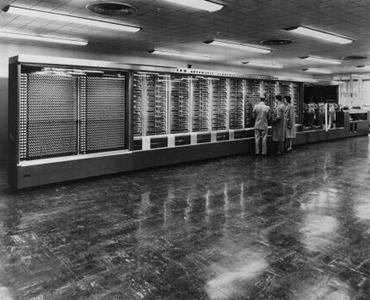
\includegraphics[width=.75\linewidth]{./Imagenes/ascc.jpg}}
		\caption{ASCC}
		\label{fig:ascc}
	\end{subfigure}%
	\begin{subfigure}{.5\textwidth}
		\centering
		\href{https://www-03.ibm.com/systems/z/hardware/z13.html}{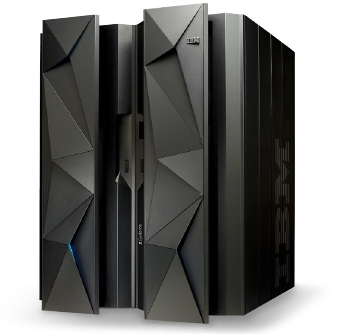
\includegraphics[width=.65\linewidth]{./Imagenes/z13.jpg}}
		\caption{\href{https://www-03.ibm.com/systems/z/}{Z13}}
		\label{fig:z13}
	\end{subfigure}
	\caption{Evolución mainframes}
\end{figure}



\subsection{IBM mainframes}
Usaremos la siguiente definición de mainframe \cite{ibm-mainframes}
\begin{center}
	$"$Un mainframe es lo que las empresas usan para alojar bases de datos comerciales, servidores de transacciones y aplicaciones que requieren un mayor grado de seguridad y disponibilidad de lo que comúnmente se encuentra en máquinas de menor escala$"$ 
\end{center}

El desarrollo de este tipo de computadoras comenzó en los años cincuenta, las grandes empresas los utilizaban como repositorios de datos.
El término evolucionó desde considerarse solamente el hardware de IBM hasta entenderse como un estilo de computación en sí mismo.
En los sesenta se comenzó a estandarizar tanto el hardware como el software.

% The introduction of the IBM System/360™ (or S/360™) in 1964 signaled the start of the third generation: the first general purpose computers.
% En el otro enlace pone que el primero fue ASCC (?)
\

Un punto de inflexión en la historia fue el \textit{S/360}, el primero de estos ordenadores en usar microcódigo para muchas instrucciones máquina, sin tener todas sus instrucciones cableadas. 
El microcódigo (o firmware) consiste en microinstrucciones (no disponibles para los usuarios) que proporcionan una capa funcional entre el hardware y el software, nos ofrece flexibilidad ante cambios sin tener que reemplazar el hardware.
Las primeras aplicaciones empresariales se programaron en ensamblador, COBOL, FORTRAN o PL/1, y muchos de estos programas todavía siguen en uso.

\subsubsection{Arquitectura}
A principios de los noventa el modelo de nodos menos potentes distribuidos emergió para desafiar el dominio de los mainframe, por aquel entonces eran llamados dinosaurios.
Los diseñadores desarrollaron nuevos mainframes llamados T-Rex, algunos de los servicios que ofrecían eran el servicio web, mayor autonomía, recuperación ante desastres y computación grid.
La computación grid hace referencia al uso simultáneo de diferentes recursos hardware y software cumpliendo varias características \cite{grid-def}:

\begin{minipage}{\linewidth}
	\centering
	\begin{minipage}{0.45\linewidth}
		\begin{itemize}
			\item Coordinar recursos de forma descentralizada
			
			\item Protocolos e interfaces estándares, abiertos y de propósito general
			
			\item Ofrecer un servicio no trivial
		\end{itemize}
	\end{minipage}
	\hspace{0.1cm}
	\begin{minipage}{0.45\linewidth}
		\begin{figure}[H]
			\centering
			\label{grid-c}
			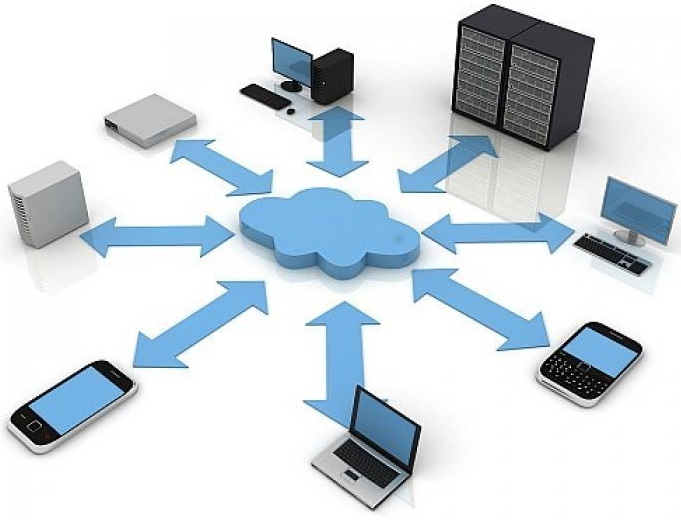
\includegraphics[width=0.7\textwidth]{./Imagenes/grid-c.jpg}
			\caption{Computación grid, \href{http://tongdaiao.com.vn/tong-dai-ao-la-su-hien-dien-cua-mot-doanh-nghiep-thanh-cong/}{imagen}}
		\end{figure}
	\end{minipage}
\end{minipage}

\

% What is a mainframe? It's a style of computing
Hoy en día se utiliza más el término servidor, cuando tenemos un grupo lo llamamos granja y mainframe hace referencia a los servidores más grandes.
Un mainframe a menudo implica una centralización de la computación, aunque una empresa grande puede distribuir sus servicios en varios servidores.
Los mainframes tienen la capacidad de configurarse dinámicamente, añadir procesadores, memoria y conexiones, mientras las aplicaciones continúan ejecutándose.
Cuando usamos un mainframe tenemos mayor flexibilidad y evitamos actualizar varios computadores a la vez, sin embargo, tener varios computadores distribuidos aumenta la potencia de cálculo en relación al precio.

\

A menudo se utiliza el término plataforma para referirse al conjunto de hardware y software. El mainframe en sí suele cumplir varias de las siguientes características \cite{ibm-mainframes}:
\begin{itemize}
	\item Compartir acceso disco con otros sistemas, con protección de los datos y control de privilegios.
	\item Procedimientos sistemáticos de copias de seguridad y recuperación desde otra ubicación.
	\item Trabajo rutinario con operaciones simultáneas de E/S. %
	\item Permitir usar varias copias del sistema operativo como un único sistema, dicha tecnología se conoce como \href{https://www-03.ibm.com/systems/z/advantages/pso/}{Parallel Sysplex} (cluster en UNIX).
	\item Gran capacidad de compartir datos y recursos.
\end{itemize}

\

% Who uses mainframes and why do they do it?
% Mainframe strengths: Reliability, availability, and serviceability
Las fortalezas del mainframe se representan mediante las siglas RAS (Reliability, Availability y Serviceability)
\begin{itemize}
	\item Confiabilidad: El hardware tiene comprobación y recuperación de errores y se aplican actualizaciones software cuando existe un problema. 
	\item Disponibilidad: Capacidad de reemplazamiento del hardware y el software, aunque es deseable mantener un MTBF (Mean time between failure) lo más alto posible.
	\item Utilidad: Entender el tipo de los errores, lo que permite conocer lo que hay que modificar.
\end{itemize}
Otra cualidad deseable es la escalabilidad, capacidad de mantener niveles de rendimiento al agregar procesadores, memoria y almacenamiento.

\

% Mainframe strength: Continuing compatibility
% Mainframe workloads: Batch and online transaction processing
Un mainframe suele realizar dos tipos de trabajo, procesamiento en segundo plano (scripts) o transacciones online, diferenciándose en la interacción con el usuario final.

\begin{figure}[H]
	\centering
	\label{workloads}
	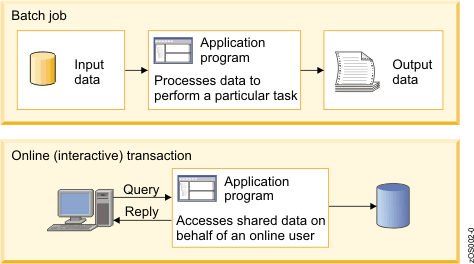
\includegraphics[trim = 0mm 0mm 5mm 0mm, clip, width=0.55\textwidth]{./Imagenes/workloads.png}
	\caption{Tipos de trabajo en un mainframe \cite{ibm-mainframes}}
\end{figure}

% Mainframe hardware concepts
\subsubsection{Hardware}
Además del grupo de procesadores primarios, los mainframes tienen una red de microprocesadores especiales que controlan el sistema.
IBM utiliza el término CPC (Central Processor Complex) para referirse a la colección física de hardware que incluye almacenamiento principal, uno o más procesadores centrales, temporizadores y canales.
A parte del procesador central un mainframe tiene un asistente SAP (System Assistance Processor) para las operaciones de entrada y salida.
Las unidades de disco físicas son unidades de tipo SCSI aunque se puede utilizar SSA, para un acceso más rápido a los discos, suele usar un RAID 5.

\

El mainframe se divide en diversas partes lógicas, cada una puede soportar un sistema operativo.
Se pueden distribuir los recursos entre las partes lógicas o usar el algoritmo interno de distribución de carga.
El software que se necesita para un mainframe suele ser muy caro, de hecho a veces un cliente quiere el último mainframe y más lento, para reducir costes software (el software suele ir en función de la potencia) \cite{ibm-mainframes}.
De hecho los mainframes tienen varios procesadores que no conmutan para la potencia en las licencias software, por ejemplo: Integrated Facility for Linux (IFL), zAAP, zIIP, Integrated Coupling Facility (ICF), también tienen procesadores de repuesto, llamados Spare. 
De hecho se llega a controlar la potencia de los procesadores principales insertando ciclos nulos en la secuencia de instrucciones del procesador.
Cada procesador tiene $8KB$ compartidos para PSA (Prefix Storage Area) y se utiliza para el manejo de interrupciones y de errores.

\

% Clustering on the mainframe: Parallel Sysplex and other techniques
La más sofisticada de las técnicas de clustering es \href{https://www.ibm.com/support/knowledgecenter/zosbasics/com.ibm.zos.zmainframe/zconc_clusterPlSys.htm?view=embed}{Parallel Sysplex}, permitiendo enlazar hasta 32 servidores con escalabilidad casi lineal, pero hay otras técnicas, entre ellas \href{https://www.ibm.com/support/knowledgecenter/zosbasics/com.ibm.zos.zmainframe/zconc_clusterDASD.htm?view=embed}{Basic shared direct access storage devices (DASD)} y  \href{https://www.ibm.com/support/knowledgecenter/zosbasics/com.ibm.zos.zmainframe/zconc_clusterCTC.htm?view=embed}{Channel-to-channel (CTC) rings}.


\subsection{Watson}
En 2007 \href{https://www.research.ibm.com/}{IBM Research} se propuso el reto de crear un sistema para competir con los grandes campeones en el juego \href{https://www.jeopardy.com/}{Jeopardy!}. 
Este sistema, en adelante Watson, entraría dentro de la categoría QA (Question answering), que engloba varias áreas de la ciencia de la computación y la inteligencia artificial. 
Algunas de estas áreas serían búsqueda y recuperación de información (IR), procesamiento de lenguaje natural (NLP), representación del conocimiento y razonamiento o el machine learning.

\begin{figure}[H]
	\centering
	\label{j-watson}
	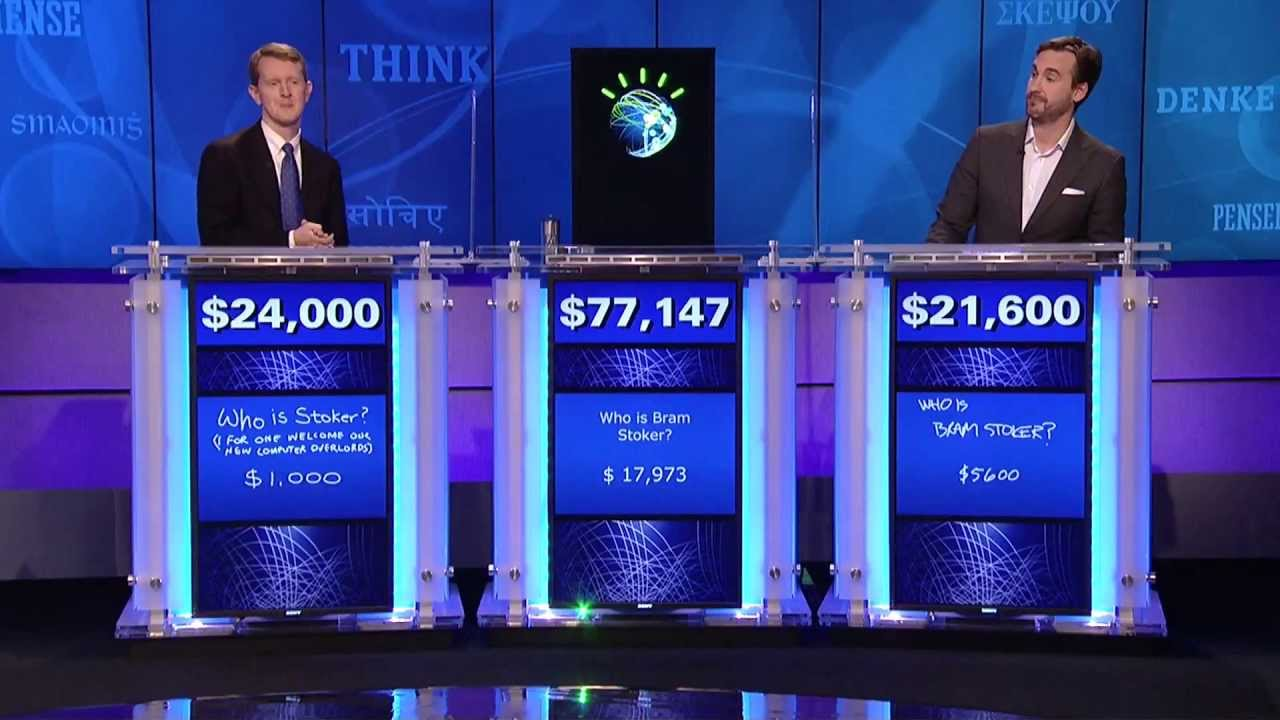
\includegraphics[width=0.8\textwidth]{./Imagenes/j-watson.jpg}
	\caption{Watson en Jeopardy!}
\end{figure}

\

La comunicación humana es imperfecta, el lenguaje permite ambigüedades, polisemia, la misma información puede expresarse de varias formas, también tenemos ironías y la interpretación de una frase puede depender de conversaciones anteriores entre los interlocutores.
Además, dicha comunicación no está estructurada (como en un lenguaje de programación o una base de datos), los datos no siempre están bien definidos y hay información implícita.
A día de hoy la información no estructurada crece muy rápido, por ello es buena idea desarrollar el análisis del lenguaje natural y hacer inferencia a partir de los datos de los que disponemos.
% this-is-watson: word-sense disambiguation [5, 6], latent semantic analysis [7], textual entailment [8], and coreference resolution [9]

\

Desde 2001 hasta 2006 se construyó la base para el reconocimiento de información no estructurada, UIMA (Unstructured
Information Management Architecture). % this-is-watson:[10]
UIMA proporciona una plataforma para integrar la información obtenida tras analizar textos, imágenes, etc.
Su objetivo es integrar varios programas llamados \textit{anotadores}, que asignan significado semántico a ciertas partes del texto o imagen.

% Watson was the system-level experiment that brought together hundreds of different cooperating algorithms, each of these algorithms alone performs relatively simple language processing tasks.
% In May 1997, IBM’s Deep Blue* computer beat Gary Kasparov (IBM Research beckoned for an encore)
\

Algunos desarrolladores habían participado anteriormente en Question answering dentro del proyecto PIQUANT \cite{piquant}. % this-is-watson [13, 14]
Este sistema tenía un conjunto estático de tipos de respuestas (o clases de conceptos) que se solicitaban en una pregunta.
El nuevo sistema no tendría conexión a Internet, y tendría que procesar la pregunta, buscar respuesta y estimar la probabilidad de que sea correcta.
Tras analizar $2.000$ partidas de \textit{Jeopardy!} la media de los jugadores que ganaban era una precisión del $85-95\%$ de acierto sobre una media de $40-50\%$ de preguntas respondidas, o 
\textit{85\% Precision@40}.
En $2007$ se consiguió, usando PIQUANT, un rendimiento \textit{16\% Precision@70} en las preguntas de \textit{Jeopardy!}.


\subsubsection{Arquitectura}
Sobre UIMA se desarrollaron dos técnicas esenciales en el desarrollo de \textit{Watson}, la arquitectura DeepQA % this-is-watson: [4]
y un complemento para integrar distintas técnicas algorítmicas llamado AdaptWatson. % this-is-watson: [16,17]

\begin{figure}[H]
	\centering
	\label{tiw-deepqa}
	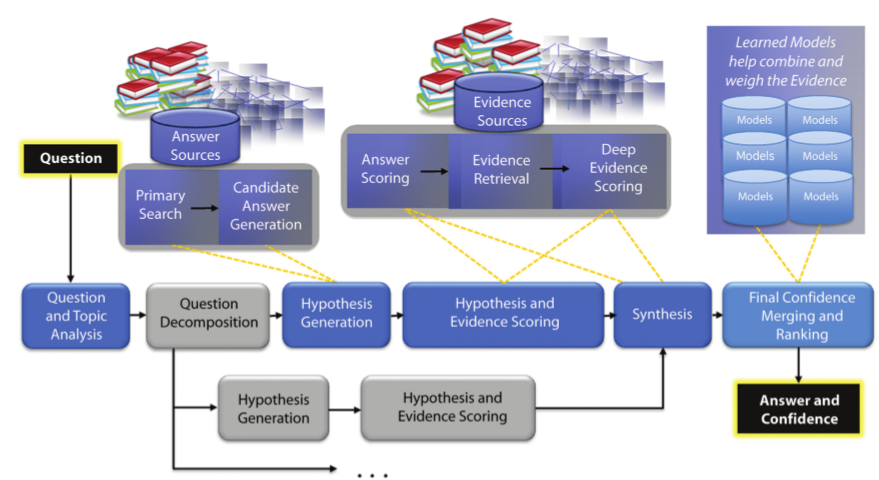
\includegraphics[width=0.8\textwidth]{./Imagenes/deepQA.png}
	\caption{Arquitectura DeepQA}
\end{figure}

\textbf{DeepQA} define varias etapas del análisis, cada una tiene diferentes implementaciones que se ejecutan en paralelo y se combinan los resultados.
No se presupone que se ha entendido una pregunta, de forma que pueda consultarse directamente la respuesta en nuestra base de conocimiento.
Lo que se hace es generar varias preguntas candidatas, generar varias respuestas por pregunta candidata y estimar la probabilidad de que cada respuesta sea correcta.

\

Se le da valor al hecho de que una respuesta concuerde con el tipo que se espera, por ejemplo un monumento histórico, una persona, etc.
También se tienen en cuenta fechas, geografía, la fiabilidad de las fuentes, etc.
Este análisis produce cientos de valores o características, cada uno indicando el grado de evidencia dada una respuesta concreta.
Con esas características se calcula la probabilidad de que una respuesta sea correcta dada una pregunta candidata.
Para ponderar el valor de cada característica se entrenó un modelo estadístico usando machine learning a partir de preguntas y respuestas anteriores.
% this-is-watson: [37]

\

El rendimiento del sistema era bajo por lo que se integraron diferentes técnicas algorítmicas y se añadió una metodología llamada \textbf{AdaptWatson}.
Estos componentes actúan sobre la arquitectura de DeepQA con el objetivo de entender las preguntas, buscar respuestas candidatas y valorar las respuestas.
El equipo documentó más de $8.000$ experimentos independientes, cada uno con $10-20GB$ de datos.
A partir de estos datos se buscaban fallos y sus posibles causas, de esta forma se mejoró hasta un \textit{85\% Precision@70}.

\subsubsection{Entendiendo las preguntas}
Cada pregunta en \textit{Jeopardy!} tiene una categoría que ayudará a ponderar las respuestas. % this-is-watson: question analysis algorithms [18]
Para entender las preguntas formuladas se usa un parser ESG (English Slot Grammar) % this-is-watson: [19]
y un generador PAS (predicate-argument structure). 

\begin{itemize}
	\item ESG identifica partes de la frase y roles sintácticos como el sujeto y relaciones entre las diferentes partes de la frase.
	\item El generador PAS crea una representación abstracta, la interfaz con la parte analítica.
\end{itemize}

Para las \textbf{respuestas y fuentes de evidencia} se añadieron enciclopedias y libros de referencia. Después se desarrolló un proceso semiautomático para aumentar la base de conocimiento, añadir contenido sin parar afecta negativamente al rendimiento del sistema.
% this-is-watson: proceso para añadir conocimiento [20, 21]
Para extraer conocimiento de las fuentes seleccionadas se usa \textit{PRISMATIC} \cite{prismatic}. %*
% this-is-watson: descubrir respuestas candidatas [22]

\

Cada una de las consultas usa simultáneamente información estructurada y no estructurada .
% this-is-watson: generación de hipótesis [23]
Una métrica %(candidate binary recall)
que se usa para medir la bondad de una respuesta es el porcentaje de preguntas en las que dicha respuesta es generada como candidata. 
Esta medida ayuda sobre todo cuando tenemos varias interpretaciones diferentes de la pregunta.
De las experiencias con \textit{PIQUANT} se sabía que no era una estrategia adecuada intentar anticipar todos los tipos de respuesta y crear algoritmos que busquen solamente instancias de dichas clases.
Todo el sistema se apoyaría en reconocer correctamente el tipo de respuesta y que la respuesta esté bien clasificada dentro del sistema.
En la siguiente pregunta de la categoría \textit{decoración} el tipo de respuesta buscada es una \textit{dirección}:

\begin{center}
\textit{Si usted está de pie, es la dirección que debe buscar para ver el revestimiento.}

\textbf{Respuesta}: Abajo
\end{center}

\

Para clasificar las respuestas se usó un sistema dinámico que tenía en cuenta el contexto de la pregunta, su nombre es \textit{coacción de tipo}. % this-is-watson: [24, 27]
Otras técnicas usadas por Watson eran \textit{YAGO} y \textit{WordNet}. % this-is-watson [21, 25, 26]
Otra fase del proceso es \textbf{recolectar y evaluar la evidencia} (de forma paralela) de las respuestas. 
% this-is-watson: extracción dinámica de tipos [29]
Aquí se utiliza la deducción de relaciones semánticas a partir de datos de entrenamiento. Por ejemplo, esta pregunta de la categoría \textit{Madres e hijos}:

\begin{center}
\textit{Aunque solo les separa un año de vida, ella interpretó a la madre de Colin Farrell en Alexander.}

\textbf{Respuesta}: Angelina Jolie

\textbf{Relación}: protagoniza(ella, Alexander)
\end{center}

\

En Jeopardy! hay preguntas que tienen referencias implícitas en la frase, y unas partes del enunciado pueden depender de otras, como en el siguiente ejemplo de la categoría \textit{Antes y después}:

\begin{center}
\textit{La estrella de Jerry Maguire que mantiene automáticamente la velocidad de tu vehículo.}

\textbf{Respuesta}: Control Tom Cruise
\end{center} 

Primero se detectan este tipo de preguntas y las referencias enlazadas.
Para interpretar las preguntas se dividen en distintas partes lógicas que puedan ser exploradas independientemente y combinar los resultados. % this-is-watson: [36]
Por ejemplo, en esta pregunta con categoría \textit{Animales ficticios}, el sistema puede buscar por un lado personajes introducidos en $1894$ y por otro aquello relacionado con $"$Hindi for bear$"$:

\begin{center}
\textit{El nombre de este personaje, introducido en $1894$, proviene de $"$Hindi for bear$"$.}

\textbf{Respuesta}: Baloo
\end{center}

\

El sistema debe mejorar las $2$ horas de procesamiento que necesita para responder una pregunta (en $2008$).
El $UIMA-AS$ permite a cualquier aplicación $UIMA$ ser desplegada en  procesos asíncronos que utilizan paso de mensajes.
Cada pregunta genera varias preguntas candidatas que se ejecutan independientemente, cada respuesta potencial por pregunta se busca independientemente, y cada comprobación de evidencia también.
Tras usar $2880$ procesadores la latencia de respuesta bajó de dos horas a tres segundos. % this-is-watson [39]

\

Este sistema de pregunta-respuesta es estático y no aprovecha todo el potencial de la arquitectura DeepQA.
Watson puede aplicarse a la salud modificando su base de conocimiento y enseñándole a hacer las preguntas adecuadas a los pacientes para obtener información sobre ellos e inferir una solución a partir de su historial médico.

\subsubsection{Evolución del sistema}
Watson en la actualidad no solamente se utiliza aplicado a la medicina, también se usa en finanzas e inteligencia de negocio en general.

\begin{figure}[H]
	\centering
	\label{watson2today}
	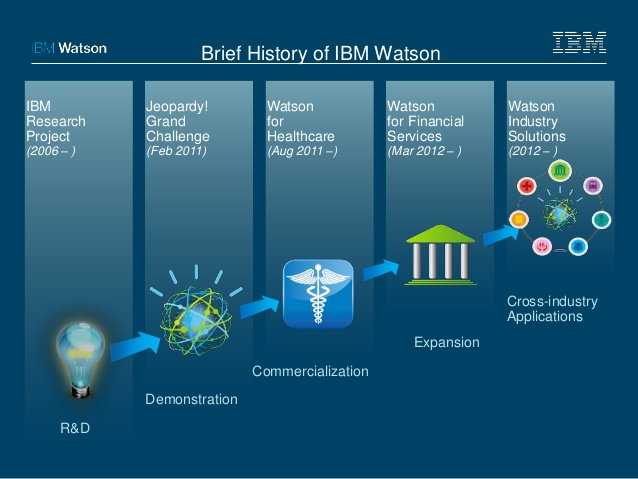
\includegraphics[trim = 0mm 14mm 0mm 10mm, clip, width=0.8\textwidth]{./Imagenes/watson2today.jpg}
	\caption{Evolución del sistema Watson \cite{watson-history}}
\end{figure}



\subsection{IBM Bluemix}
\href{https://www.ibm.com/cloud-computing/bluemix/es/node/2041}{IBM Bluemix} \cite{bluemix-doc} es una plataforma de cloud computing que combina la \href{https://azure.microsoft.com/es-es/overview/what-is-paas/}{plataforma como servicio (PaaS)} con la \href{https://azure.microsoft.com/es-es/overview/what-is-iaas/}{infraestructura como servicio (IaaS)}.

\begin{figure}[H]
	\centering
	\label{ibm-bluemix.jpg}
	
\includegraphics[width=0.45\textwidth]{./Imagenes/ibm-bluemix.jpg}
	\caption{Logo IBM Bluemix \cite{bluemix-image}}
\end{figure}

\

Bluemix integra servicios que hacen uso de Watson como reconocimiento de lenguaje natural, traducción, reconocimiento de lenguaje por voz, conversión de formatos de archivo, reconocimiento de emociones en texto escrito, reconocimiento de imágenes o agentes conversacionales. Permite además, adaptar estos servicios a múltiples contextos. Por ejemplo, si queremos un agente conversacional para controlar determinadas funciones de un coche, podemos desarrollar uno gracias a Watson que además domine el léxico de los componentes de un coche. O, en el caso del reconocimiento de emociones en texto escrito, podemos programar un bot que analice las reacciones en Twitter a un producto que acaba de lanzar nuestra compañía, pero también podemos usarlo para medir la satisfacción de nuestros clientes cuando usan el servicio técnico.

\

Bluemix permite usar demos gratuitas de estos servicios, y para este trabajo hemos probado algunas de ellas.



\subsubsection{Agente conversacional}
Nada más abrir el panel de configuración de nuestro agente conversacional nos ofrece la posibilidad de añadir \textit{intents}. Los \textit{intents} son distintos contextos de nuestra conversación. Un \textit{intent} podría ser, por ejemplo \#turn\_off. Al contexto \#turn\_off pertenecerían todas aquellas frases en las que el usuario implica que quiere apagar algo, aunque no aparezcan literalmente las palabras ``turn off'' (por ejemplo, ``stop the music'' pertenecería a este \textit{intent}). Los \textit{intents} son establecidos por el programador, y para cada uno de ellos debe introducir varios ejemplos de frases del usuario de ese tipo. Con el tiempo, Watson debería ser capaz de ampliar esa muestra y clasificar adecuadamente frases que no habían sido contempladas previamente. Este comportamiento es similar al que usó Watson en \textit{Jeopardy!} para deducir qué se pedía con una frase aunque no se dijera explícitamente.

\begin{figure}[H]
			\centering
			\label{panel.jpg}
			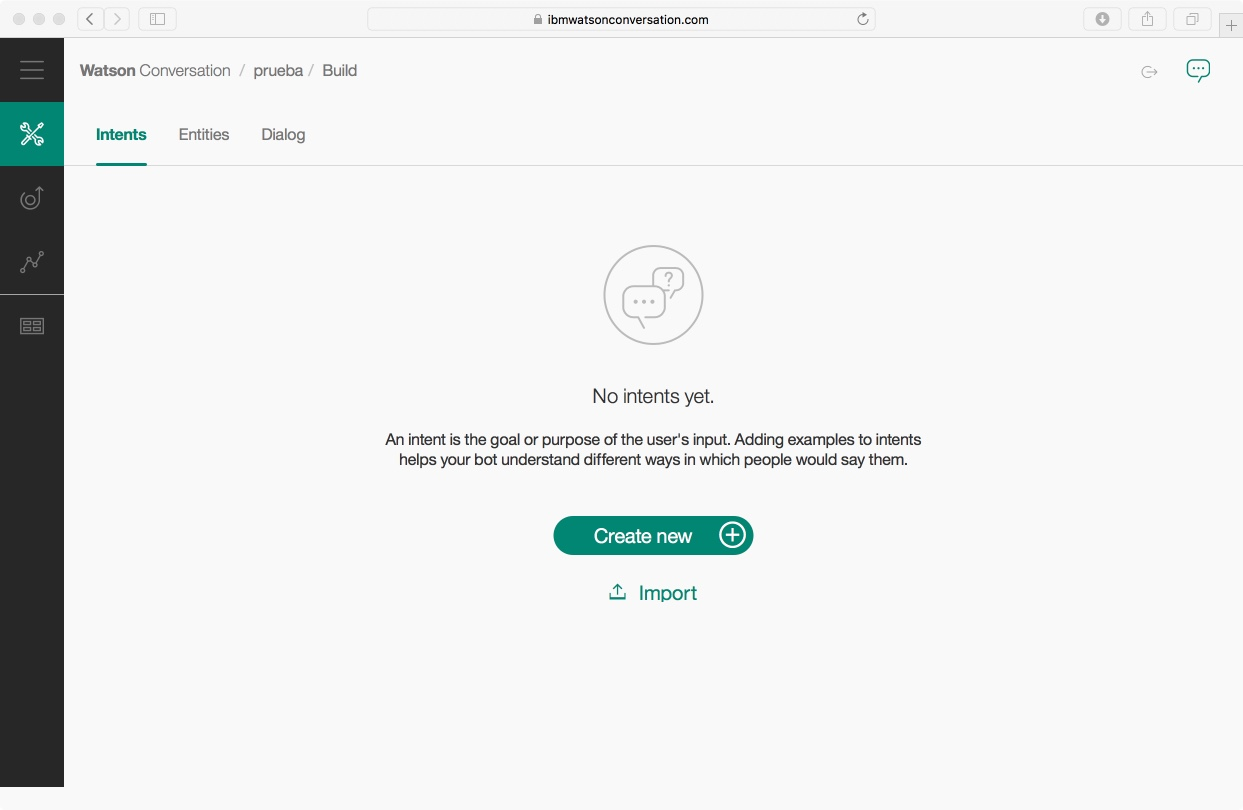
\includegraphics[width=0.75\textwidth]{./Imagenes/panel.jpeg}
			\caption{Panel para añadir \textit{intents} a nuestro agente conversacional}
\end{figure}

\begin{figure}[H]
			\centering
			\label{car1.jpg}
			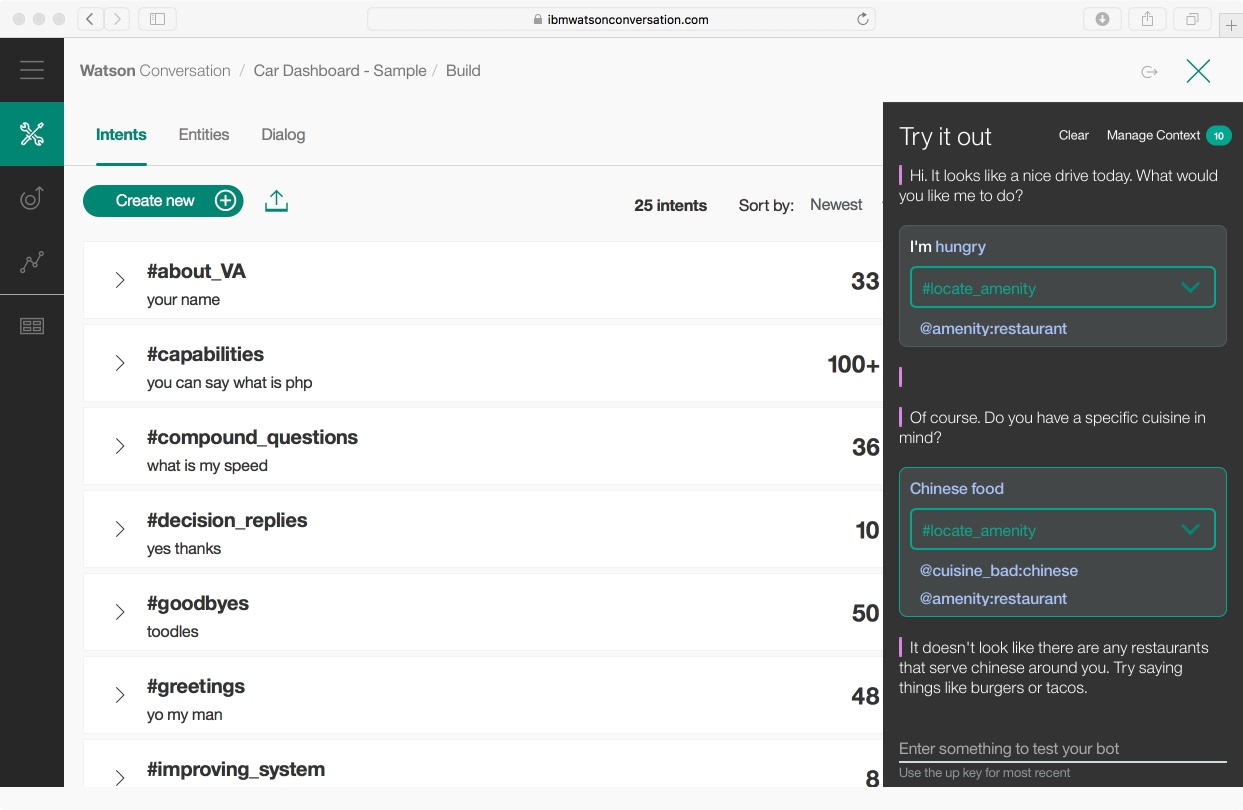
\includegraphics[width=0.75\textwidth]{./Imagenes/car1.jpeg}
			\caption{Ejemplo de un agente conversacional para asistir en la conducción (1)}
\end{figure}

\begin{figure}[H]
			\centering
			\label{car2.jpg}
			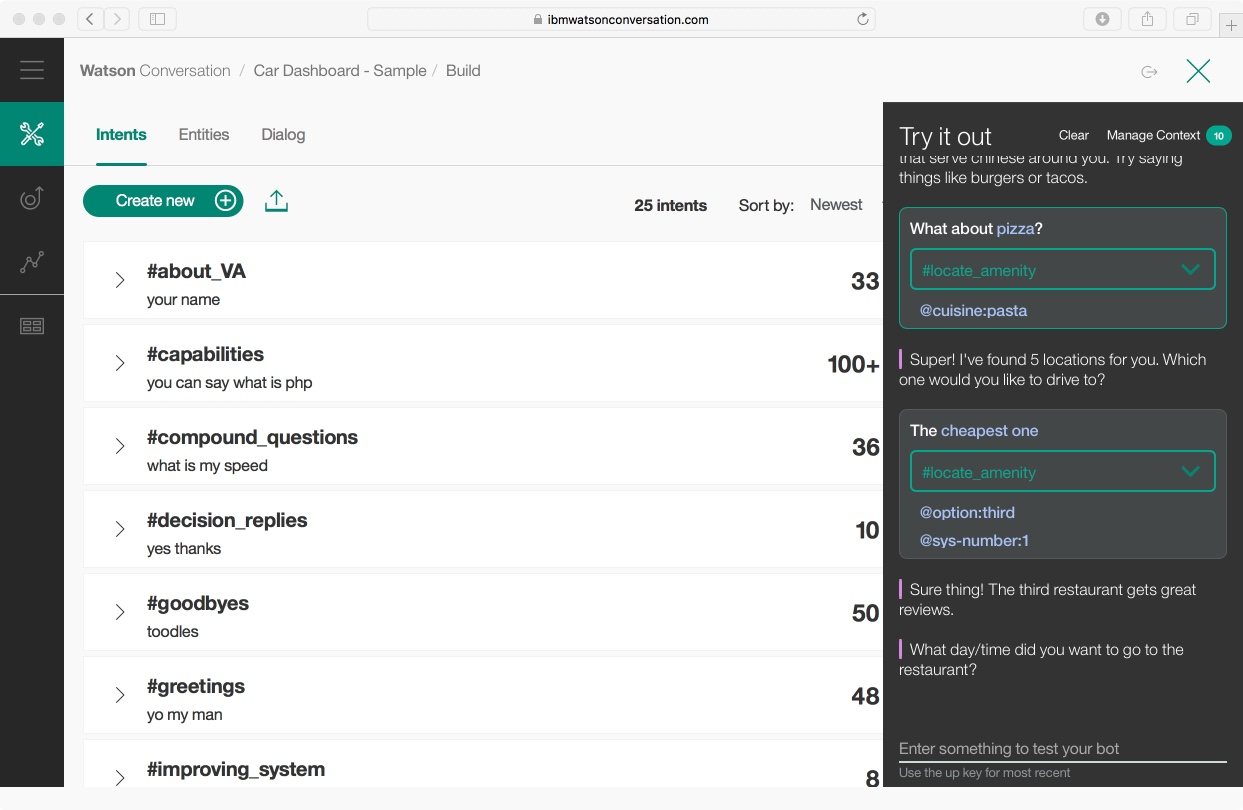
\includegraphics[width=0.75\textwidth]{./Imagenes/car2.jpeg}
			\caption{Ejemplo de un agente conversacional para asistir en la conducción (2)}
\end{figure}

\

Para el servicio de agente conversacional hemos usado una demo de un agente que será un asistente para el coche. Cuando decimos al agente ``I'm hungry'' este lo clasifica en el \textit{intent} \#locate\_amenity (``localizar servicio'') y detecta el concepto ``@amenity:restaurant'' (de nuevo, hace un uso de los conceptos similar al usado en \textit{Jeopardy!}.

\subsubsection{Detección de emociones en texto escrito}

\begin{figure}[H]
			\centering
			\label{anger.jpg}
			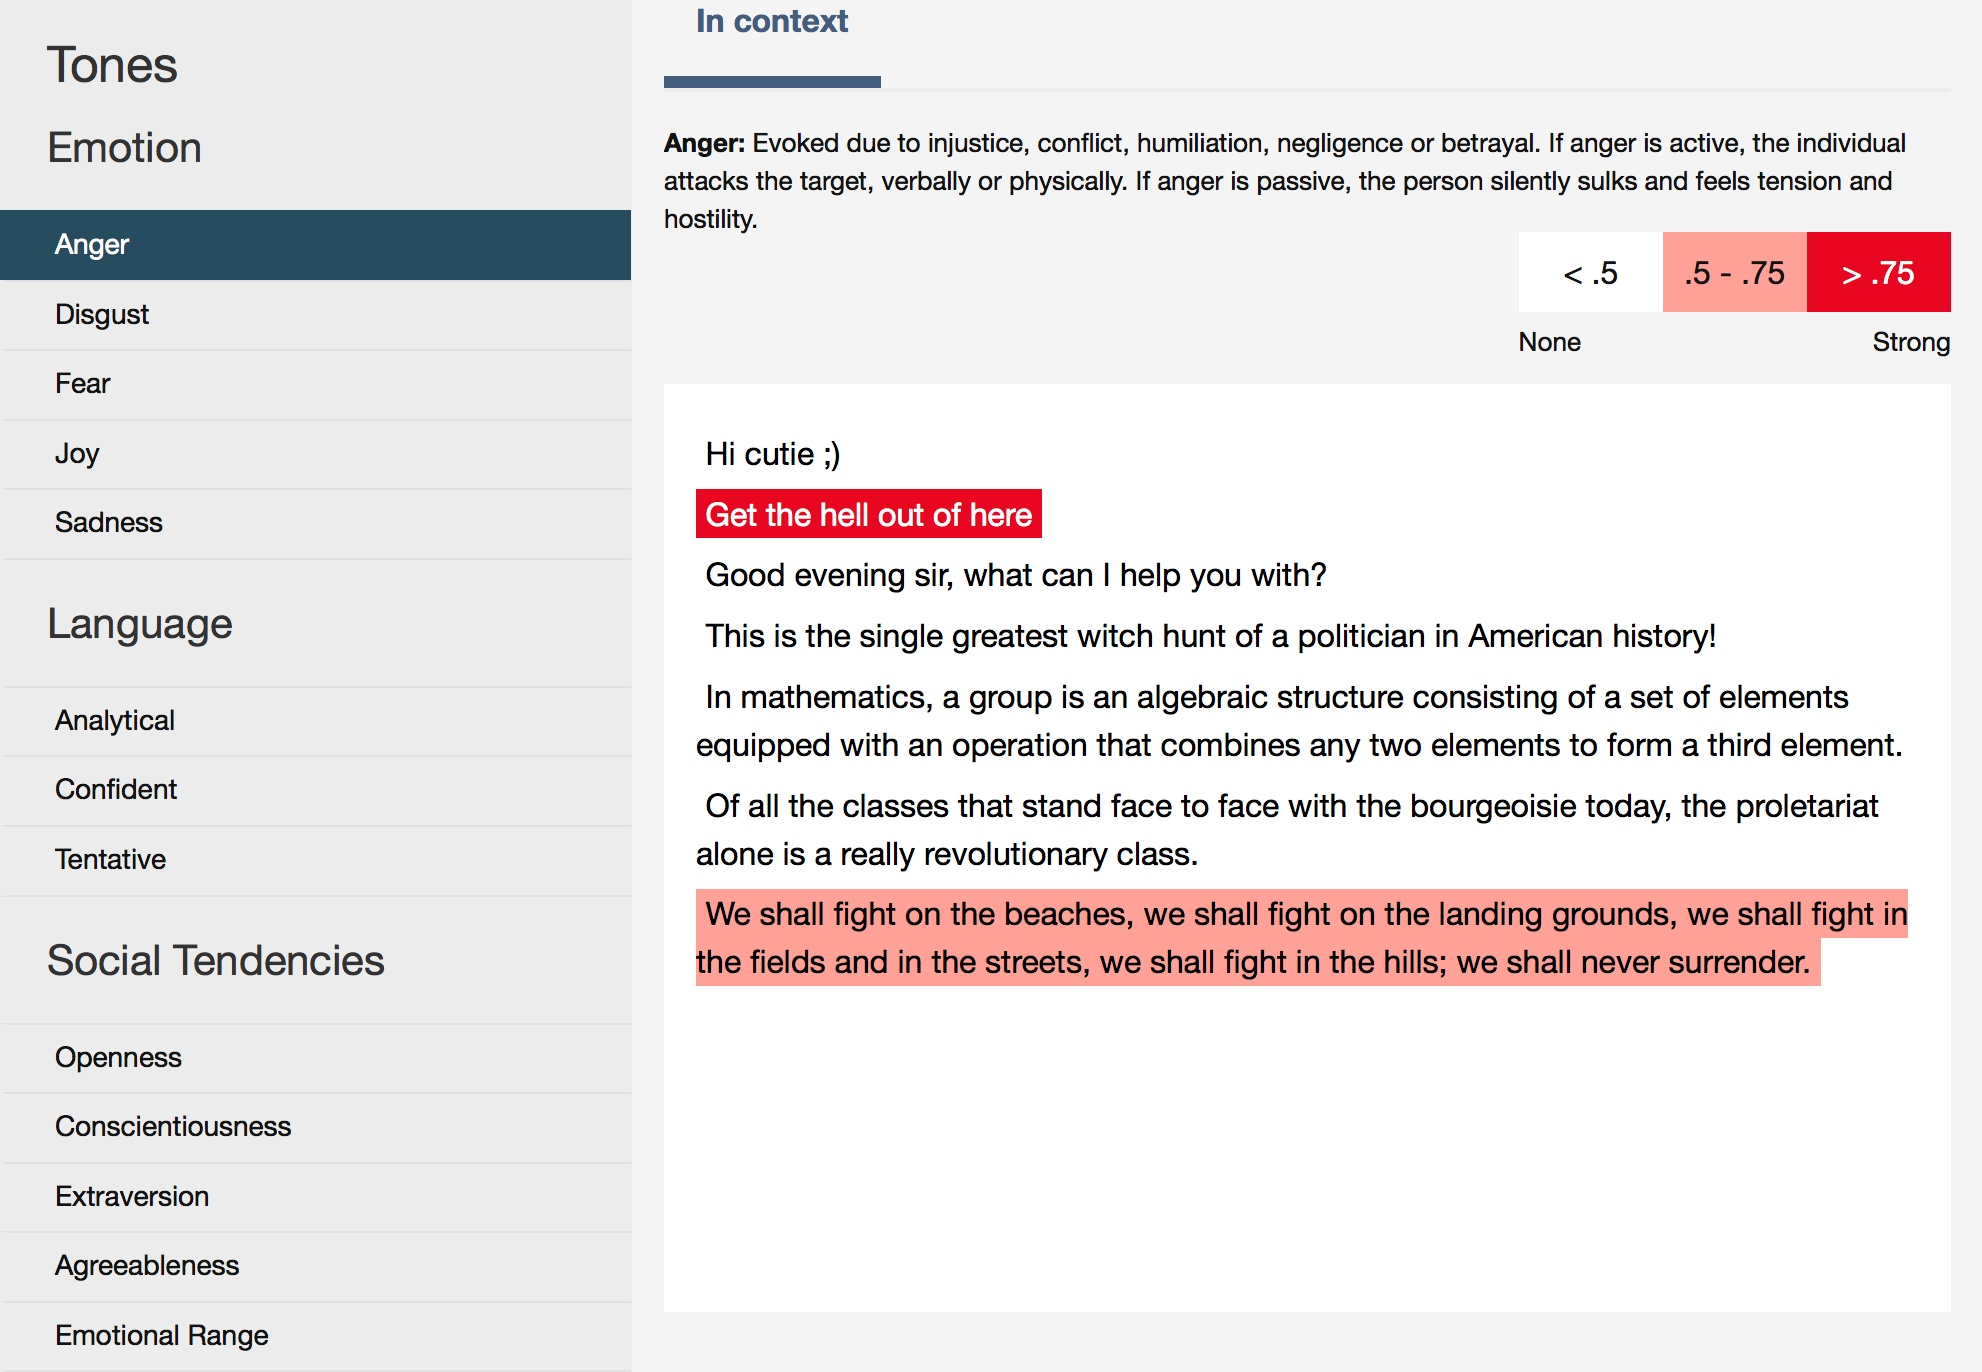
\includegraphics[width=0.75\textwidth]{./Imagenes/anger.jpeg}
			\caption{Ejemplo de detección de emociones (1)}
\end{figure}

\begin{figure}[H]
			\centering
			\label{disgust.jpg}
			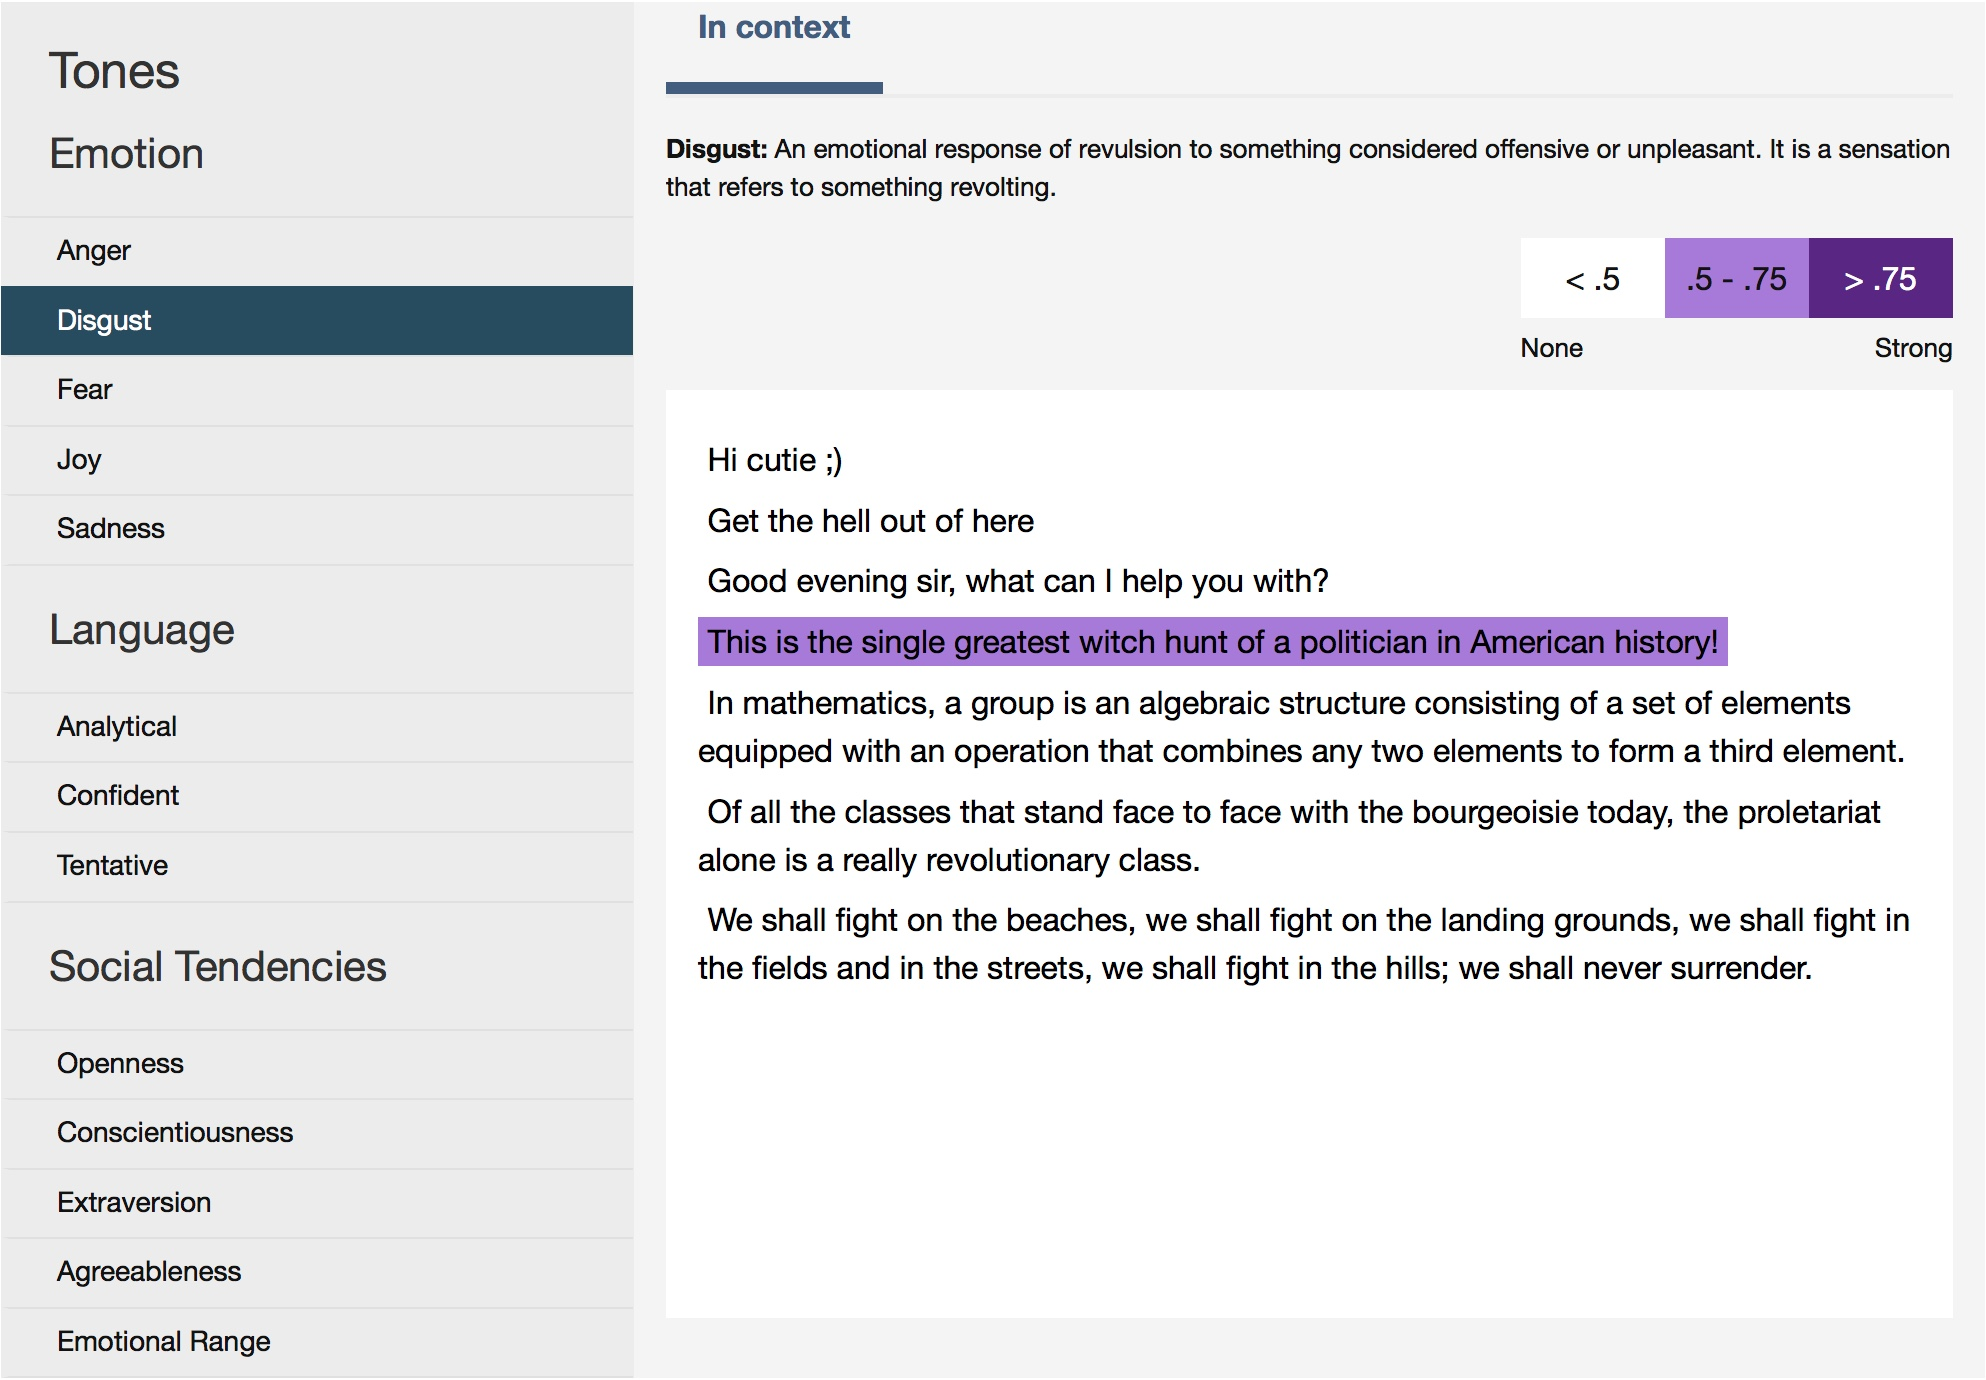
\includegraphics[width=0.75\textwidth]{./Imagenes/disgust.jpeg}
			\caption{Ejemplo de detección de emociones (2)}
\end{figure}

\begin{figure}[H]
			\centering
			\label{sadness.jpg}
			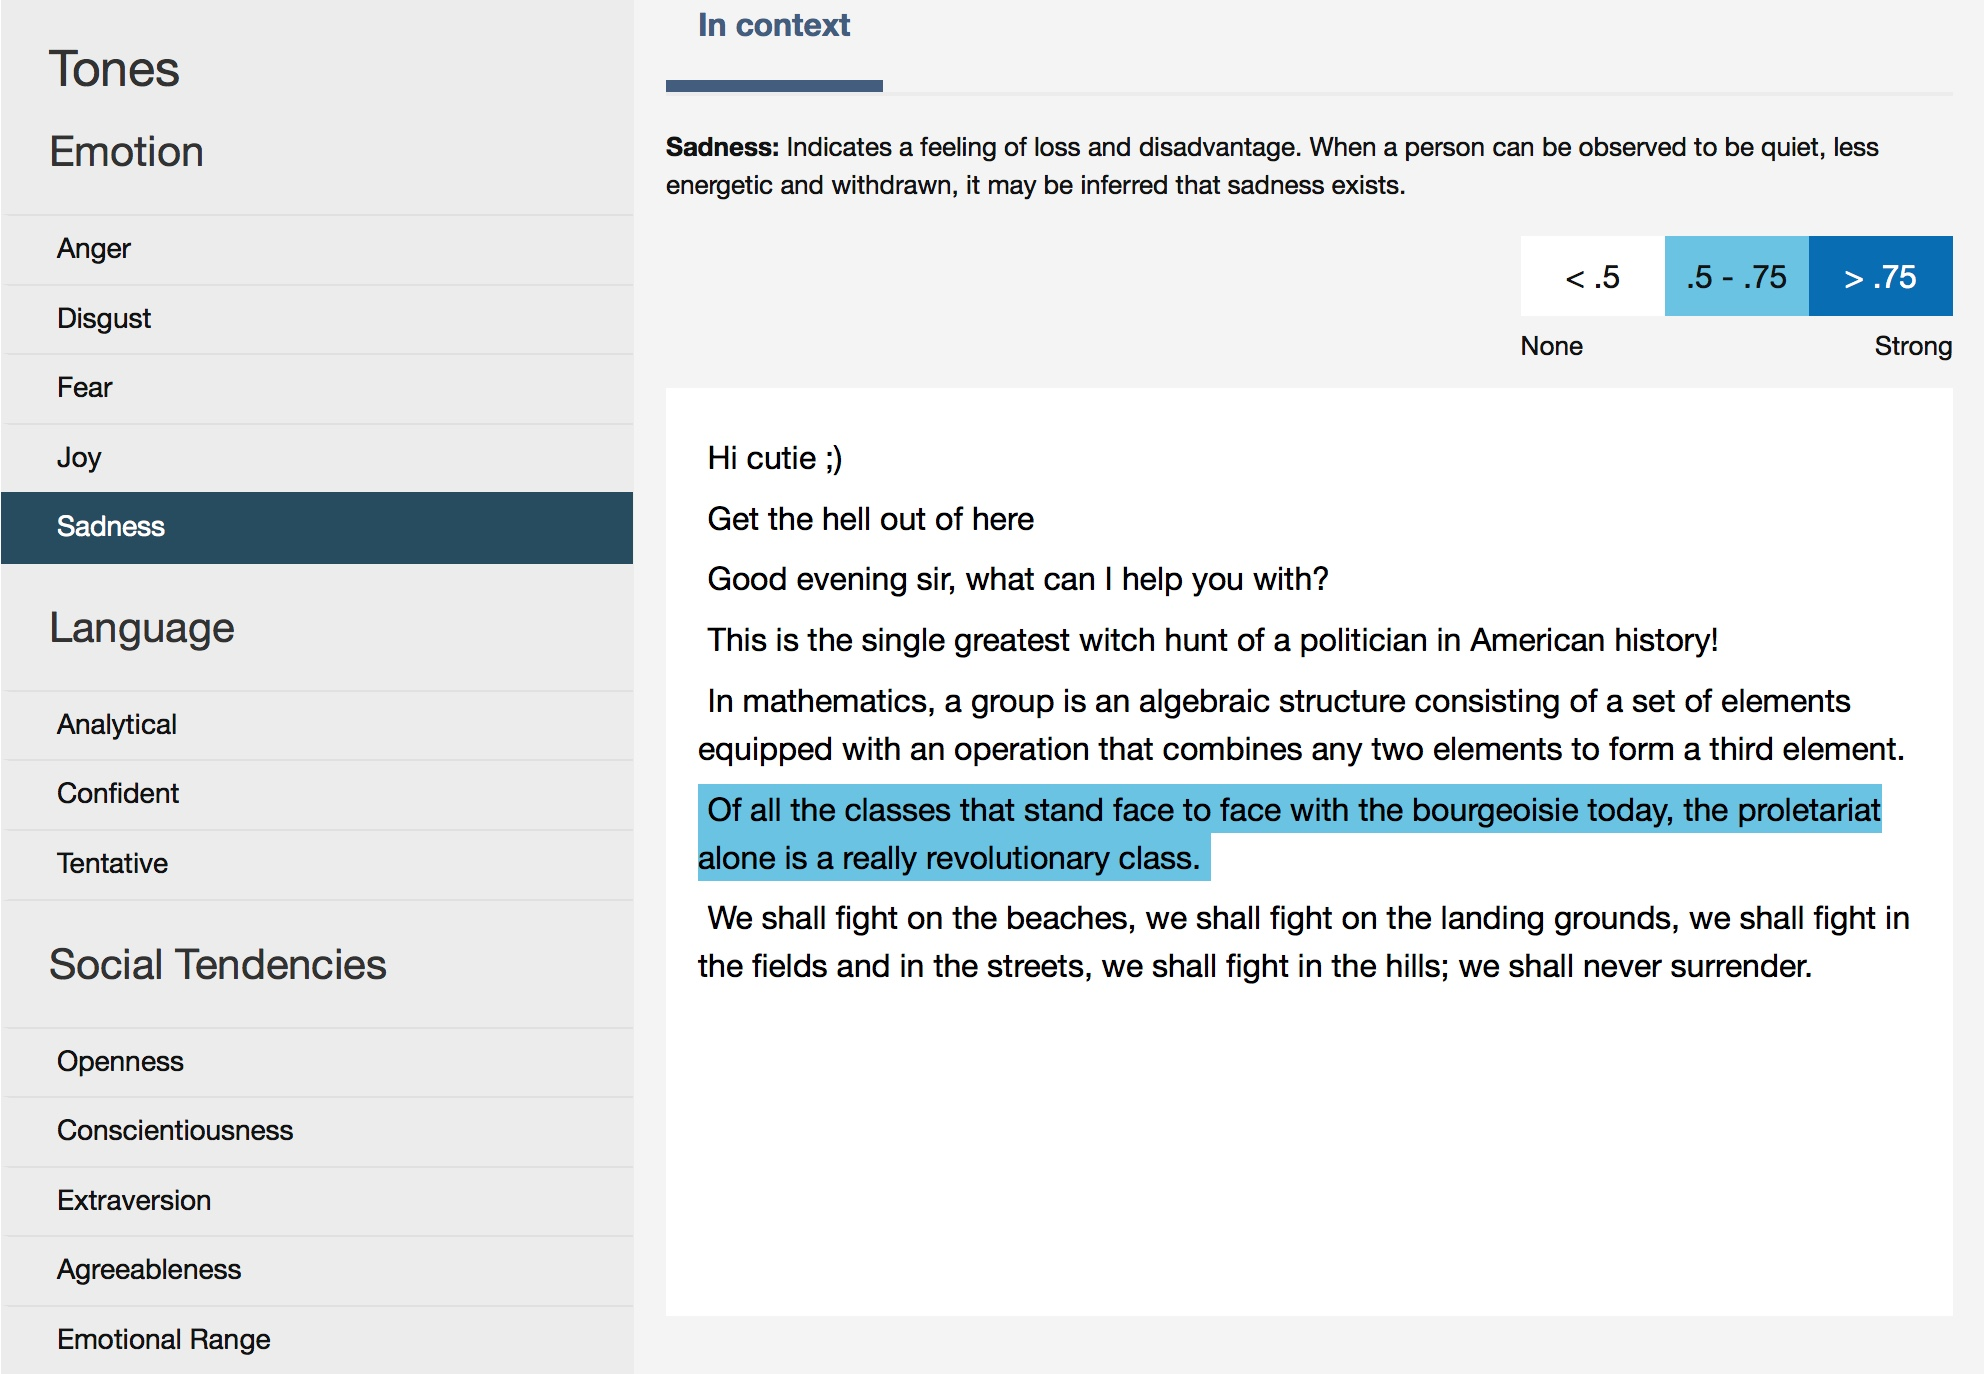
\includegraphics[width=0.75\textwidth]{./Imagenes/sadness.jpeg}
			\caption{Ejemplo de detección de emociones (4)}
\end{figure}


\begin{figure}[H]
	\centering
	\begin{subfigure}{.5\textwidth}
		\centering
		\label{conversacion1.jpg}
		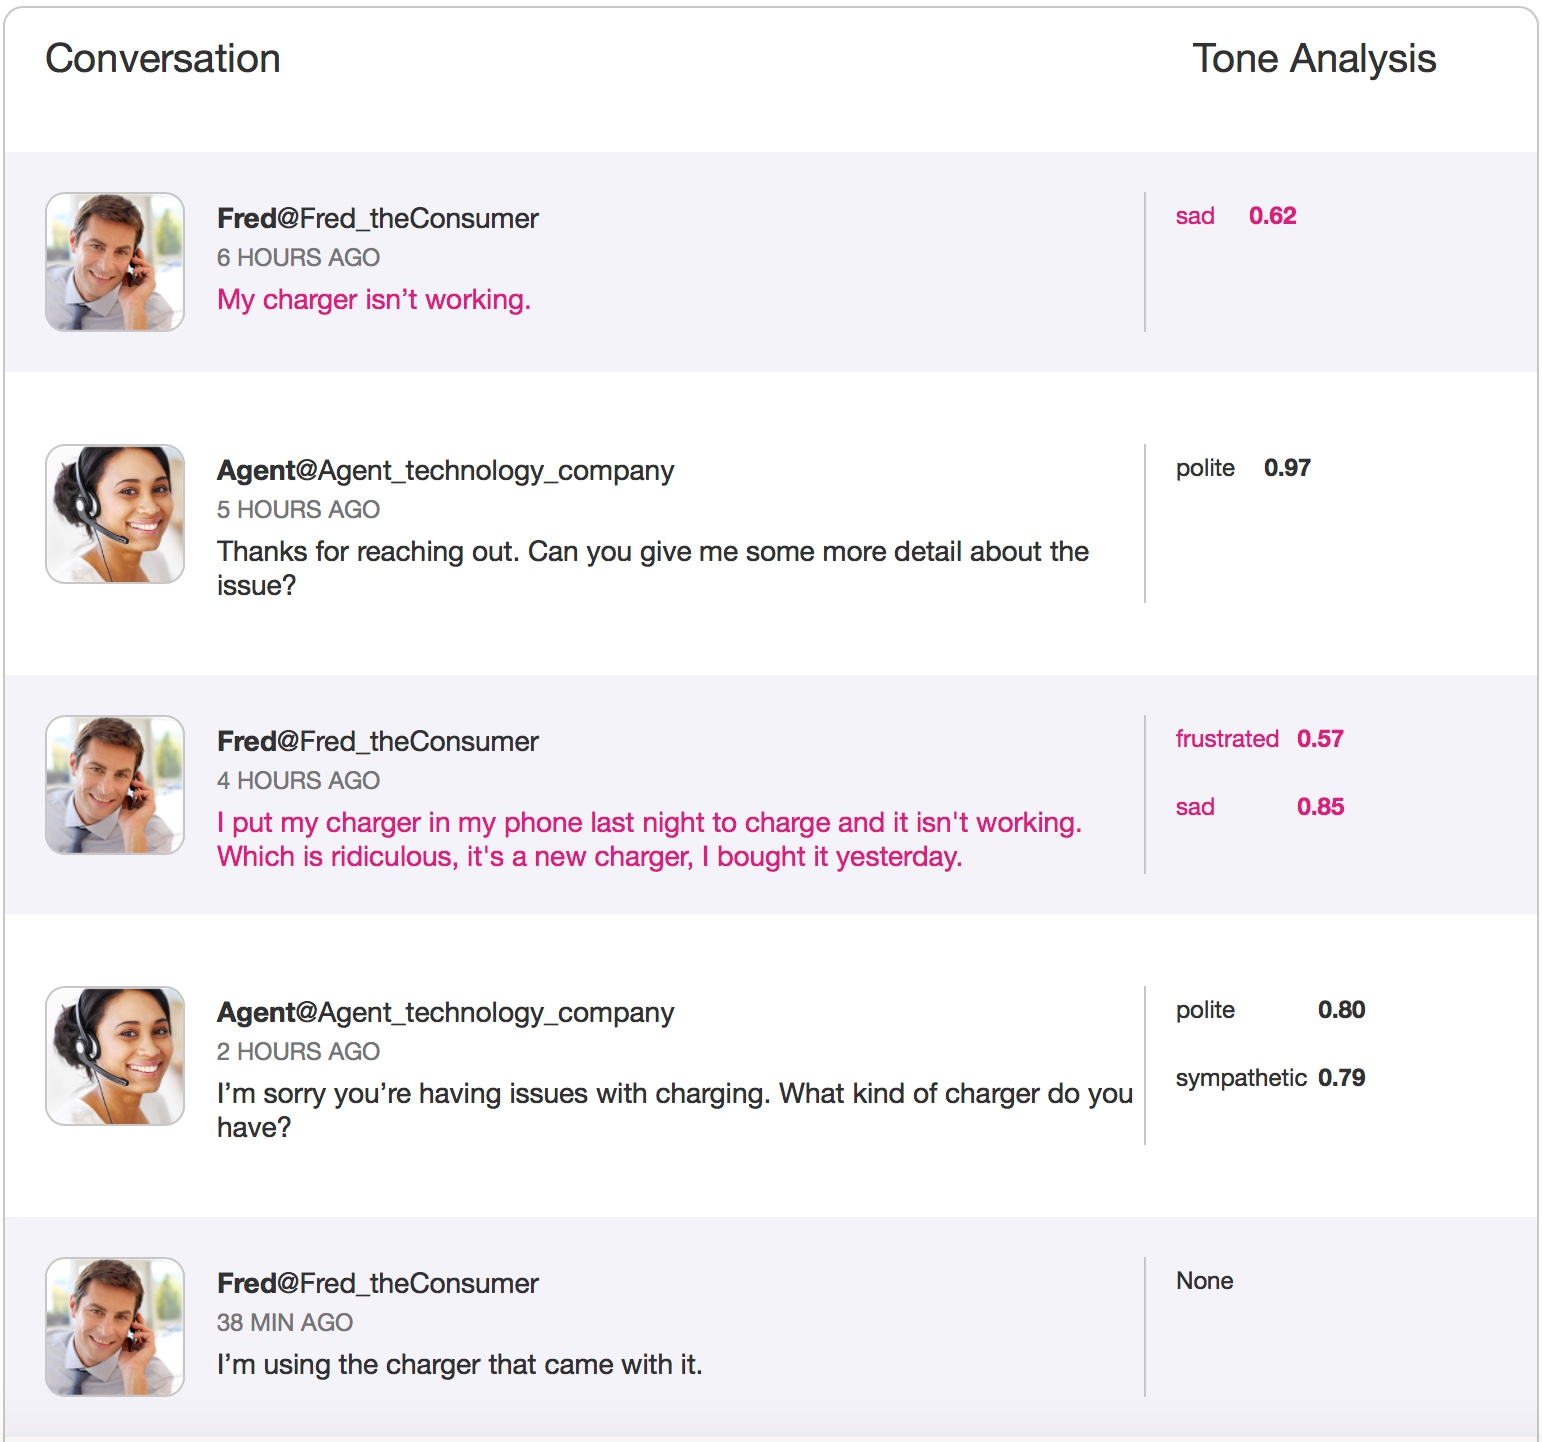
\includegraphics[width=0.99\textwidth]{./Imagenes/conversacion1.jpeg}
		\caption{Ejemplo de uso de detección de emociones para un serivicio técnico (1)}
	\end{subfigure}%
	\begin{subfigure}{.5\textwidth}
		\centering
		\label{conversacion2.jpg}
		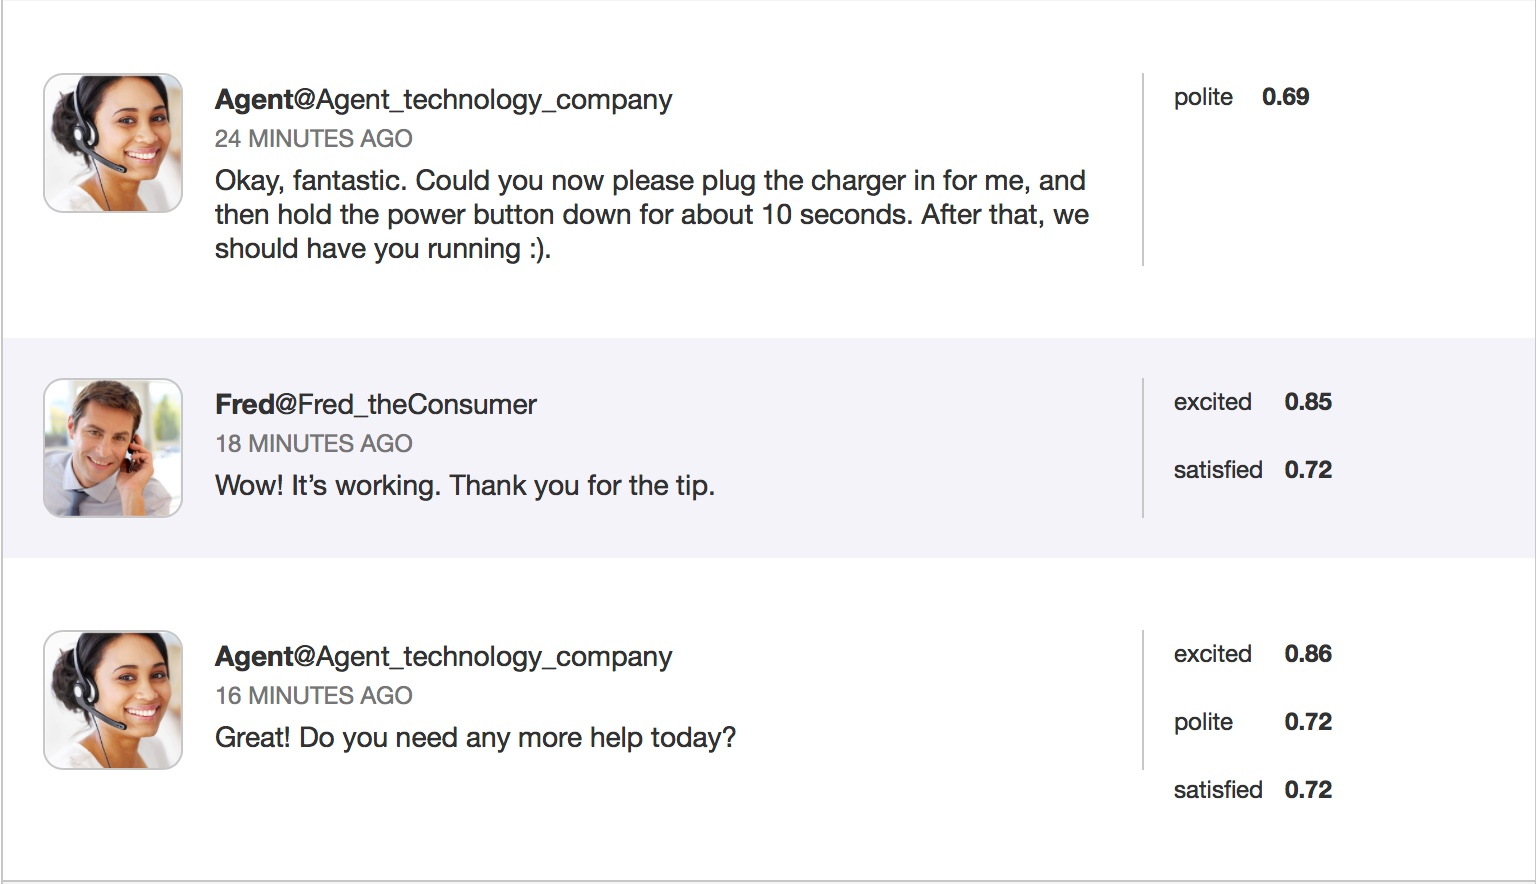
\includegraphics[width=0.99\textwidth]{./Imagenes/conversacion2.jpeg}
		\caption{Ejemplo de uso de detección de emociones para un serivicio técnico (2)}
	\end{subfigure}
\end{figure}

Otro de los servicios que ofrece Bluemix gracias a Watson es un servicio capaz de detectar emociones y tonalidad en un texto escrito. A continuación se muestran los resultados con algunas frases que hemos introducido a modo de prueba. Hemos comprobado que el análisis de las emociones que hace se basa puramente en el léxico y no tiene en cuenta demasiado la semántica. Por ejemplo, en la frase ``I hope he dies'' solo detectaba tristeza, probablemente por el uso de la palabra ``dies'', a pesar de que la frase claramente no expreza tristeza.

\

Como se ha mencionado previamente, uno de los posibles usos de este servicio es monitorizar las emociones de los clientes que hacen uso del servicio para que les sea lo más satisfactorio posible. En las siguientes figuras se muestra un ejemplo de este uso.

\section{Conclusiones}

Desde el siglo pasado, el reconocimiento del lenguaje natural ha vivido un progreso constante. Sin embargo, la victoria en 2011 de Watson en \textit{Jeopardy!} marcó un antes y un después. Empresas como IBM han sabido ver un creciente nicho de mercado en este terreno, ofreciendo servicios como traducción, reconocimiento de emociones en el texto escrito o agentes conversacionales. Lograr que un ordenador pueda mantener una conversación natural y coherente con un humano o la capacidad de reconocer el tono o la intencionalidad de las palabras es un logro que va, lógicamente, más allá de la simple satisfacción de nuestra curiosidad intelectual: el uso de estas tecnologías puede reportar beneficios para usuarios, empresas y a la sociedad en general. Los usuarios podrán tener experiencias más satisfactorias cuando contacten con el servicio técnico de un producto, controlar su casa o su coche con su voz usando expresiones naturales o hacer traducciones de calidad superior a las actuales. Las empresas podrán evaluar mejor la experiencia de sus clientes o analizar de manera más precisa las impresiones que causan sus productos. La sociedad podrá beneficiarse, por ejemplo, de mejores sistemas de salud porque seremos capaces de diseñar médicos de cabecera artificiales que analicen mejor lo que le ocurre a los pacientes, tengan acceso a cantidades ingentes de información en un instante y puedan atenderlos en sus propias casas.

\

No obstante, sigue habiendo mucho margen de mejora en el reconocimiento del lenguaje natural. Durante la prueba del servicio de reconocimiento de emociones observamos que esta tecnología deja aún mucho que desear. A menudo las interpretaciones que hacía del texto se dejaban influir por el léxico sin tener en cuenta la semántica de la frase. En el futuro se debe mejorar este aspecto, así como lograr detectar ironías o dobles sentidos. Otros retos tienen relación más directa con la ingeniería de servidores. Si queremos que los agentes conversacionales se parezcan lo suficiente a conversar con un humano, debemos mejorar los tiempos de latencia para que las respuestas sean instantáneas. Debemos ser capaces, también, de gestionar volúmenes cada vez mayores de información y extraer los datos relevantes de dicha información.


%------------------------------------------------
\newpage
\bibliography{citas} %archivo citas.bib que contiene las entradas 
\bibliographystyle{plain} % hay varias formas de citar

\end{document}
